\section{Results} 

\subsection{Fixed versus variable force field} \label{first_phase}

The experimental results are summarized in Fig. \ref{figTC}, 
in which are shown mean errors (defined as distances between the arrival point of the ball and the corresponding position of the paddle) for the two conditions \textit{Test} and \textit{Control}.

\begin{figure}[tb]
	\centering
		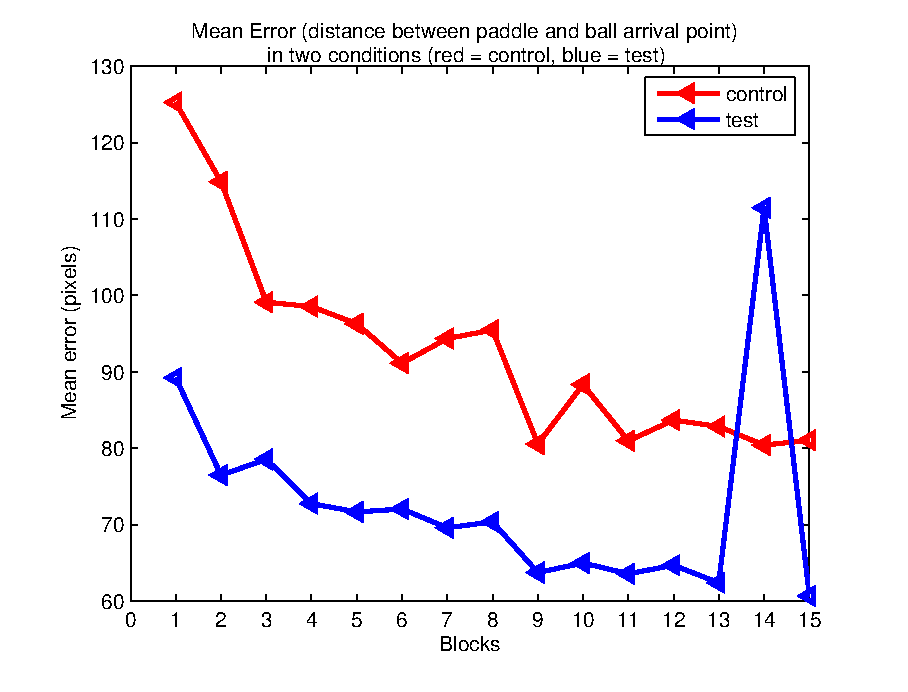
\includegraphics [width=15cm] {fig/TC.eps}
	\caption{Mean Error (distance between paddle and ball arrival point) in the two conditions (red = control, blue = test)}
	\label{figTC}
\end{figure}

The two trends appear to be well separated; in particular the latter presents a larger error during the whole experiment, with the exception of the 14th block, in which we observe a sudden error increase in the \textit{Test} condition. After this block, \textit{Test}'s error return to a value in trend with the preceding blocks. We call this particular error variation \textit{Transfer Effect}. In both conditions appears a gradual error decrease from block to block, that could suggest the existence of a common progressive learning, due, for instance to an increasing skill in using the setup.
These qualitative observation are supported by statistical analysis. An ANOVA with Condition [two levels: \textit{Test} and \textit{Control}] as a between-subjects variable, and Block [13 levels. Only the first 13 blocks of trial, in which acceleration was kept constant in the \textit{Test} condition, were taken in account] as a within-subject variable revealed significant effects of Block [\textit{p-value} $<$ .0001] and of Condition [\textit{p-value} $<$ .0001]. The Block $\times$ Condition interaction was not significant [\textit{p-value} $=$ 0.6541]. The first result, as long as a multiple comparison test, assess a significant difference in errors among the first and the later blocks of the session, therefore confirming a form of learning. Besides the significant effect of the \textit{Condition} on the results indicates that subjects get better results when the force field acting on the balls is fixed and therefore the acceleration is kept constant in all trials.

To estimate the effect of the sudden change of force field and accelerations in the 14th block of the \textit{Test} subjects, we compared the mean error of the 14th block with the mean of blocks 13th and 15th. The 14th block error results significant larger than those made in the preceding and following blocks, as assessed by a one-way ANOVA, which revealed a
significant effect of Block [2 levels] [\textit{p-value} $<$ .0001]. This result suggests that the acceleration changes, experienced by \textit{Test} subject only in this 14th block, significantly affects their performance.


\subsection{Gravitational versus anti-gravitational force field} \label{second_phase}

Afterward we analyzed separately the two sub-conditions \textit{Test - up} and \textit{Test - down}, to assess whether also the acceleration value had an influence on the error. Fig.\ref{figTTC} 

\begin{figure}[tb]
	\centering
		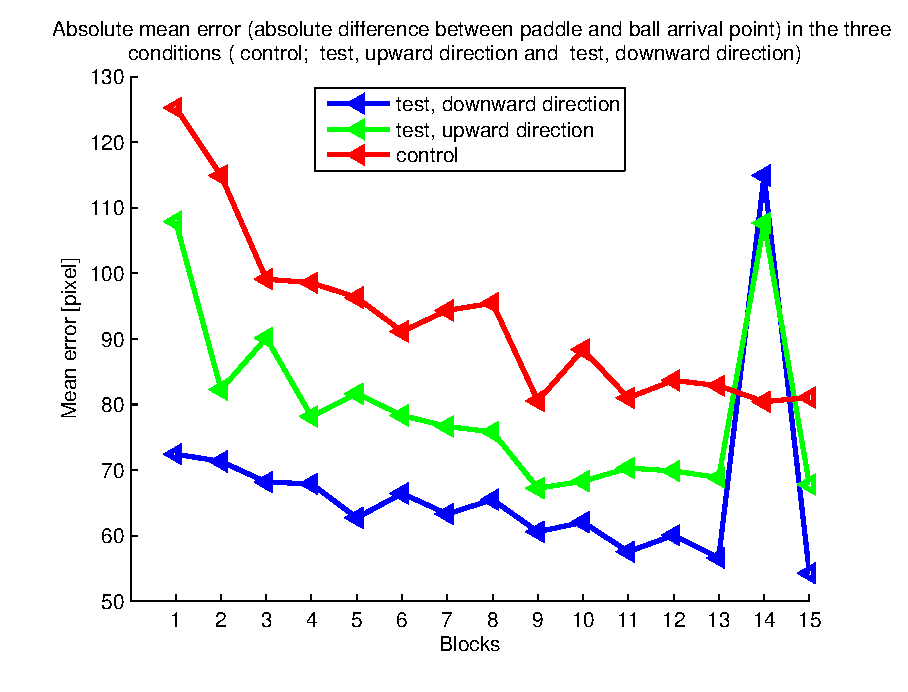
\includegraphics [width=15cm] {fig/TTC.eps}
	\caption{Mean Error (distance between paddle and ball arrival point) in the three different conditions (red = control, green = test, upward direction, blue = test, downward direction)}
	\label{figTTC}
\end{figure}



shows the mean errors for the three conditions and an almost clear separation among all of them can be observed. In all cases there is also an error decrease between the first and the later blocks.
An ANOVA with Condition [two levels: \textit{Test - up} and \textit{Test - down}] as a between-subjects variable, and Block [13 levels. Only the first 13 blocks of trial, in which acceleration was kept constant, were taken in account] as a within-subject variable revealed significant effects of Block [\textit{p-value} $<$ .0001] and of Condition [\textit{p-value} $<$ .0001], corroborating the qualitative observations suggested. The Block $\times$ Condition interaction was not significant [\textit{p-value} $=$ 0.4671].  Consequently there is a significant difference between errors of the two \textit{Test} cases too. In particular subjects who had to deal with  balls affected by a force field whose orientation was opposite to the gravitational one performed constantly worse then the other \textit{Test} group.

\begin{figure}[tb]
	\centering
		\includegraphics [width=15cm] {fig/MultCompTTC.eps}
	\caption{Multiple comparison among marginal means among errors (distance between paddle and ball arrival point) in the three different conditions (from the right control, test, upward direction and test, downward direction)}
	\label{figMultCompTTC}
\end{figure}

In order to have an overview of the results it is useful to perform a multiple comparison among the means of the three conditions errors, which supports the hypothesis of clear separation among all of them (See Fig.\ref{figMultCompTTC}).